\documentclass[10pt,twocolumn]{article}

\usepackage[table,xcdraw]{xcolor}
 \usepackage{fancyhdr}
\usepackage{array}
\usepackage{amsthm,amssymb,mathrsfs,mathtools,amsmath,dsfont}
\usepackage{titlesec}
\usepackage{color}
\usepackage[table]{xcolor}
\usepackage{xecolor}
\usepackage[a4paper, top=2.5cm, left=1.5cm,right=1.5cm, bottom=2.5cm, footnotesep=2\baselineskip]{geometry}
\usepackage{graphicx}
\usepackage{subfigure}
\usepackage{caption}
\usepackage{fontspec}
\usepackage{multicol,multirow}
\usepackage{rotating}
\usepackage[pagebackref=false,colorlinks,linkcolor=abitire,citecolor=narenj]{hyperref}


\captionsetup{belowskip=0pt,aboveskip=0pt}

\begin{document}


	
\begin{table}[!hh]
	\caption*{\textbf{Table 6.3 typical Software Process Lead Functions}}
	\begin{small}
	\begin{center}
		\begin{tabular}{|l|l|}
		\hline
		{\color[HTML]{242021} \textbf{SPL Function}}                                                                                  & \multicolumn{1}{c|}{{\color[HTML]{242021} \textbf{Function Description}}}                                                                                                                                                                                                                                     \\ \hline
		{\color[HTML]{242021} \begin{tabular}[c]{@{}l@{}}SEPG\\ Administrative\\ Chair\end{tabular}}                                  & {\color[HTML]{242021} \begin{tabular}[c]{@{}l@{}}Prepares for SEPG meetings\\  (reserveroom, agenda, etc.).\\ Prepares and distributes \\ SEPGmeeting minutes.\\ Ensures the SEPG follows\\ established applicable \\ program software processes\end{tabular}}                                                \\ \hline
		{\color[HTML]{242021} \begin{tabular}[c]{@{}l@{}}Working Group\\ Oversight\end{tabular}}                                      & {\color[HTML]{242021} \begin{tabular}[c]{@{}l@{}}Ensures that working groups\\  are effective; ensures that\\  each working group \\ understands roles,\\ responsibilities and specific\\  task assigned to the working\\  group; and monitors progress\\  of working groups, etc\end{tabular}}               \\ \hline
		{\color[HTML]{242021} \begin{tabular}[c]{@{}l@{}}Software Process\\ Improvement\\ Monitoring and\\ Appraisals\end{tabular}}   & {\color[HTML]{242021} \begin{tabular}[c]{@{}l@{}}Ensures that the appropriate\\ measurements on process\\  tasks are collected, analyzed,\\  and distributed.\\ Focal point for software \\ process appraisals\end{tabular}}                                                                                  \\ \hline
		{\color[HTML]{242021} \begin{tabular}[c]{@{}l@{}}Software Process\\ Improvement\\ Recommendation\\ Coordination\end{tabular}} & {\color[HTML]{242021} \begin{tabular}[c]{@{}l@{}}Reviews, supports and \\ presentsprocess improvement\\ recommendations from\\  program personnel, internal \\ and external groups and \\ customer, industry data on\\  current best practices,\\  companyand industry\\  standards to the SEPG\end{tabular}} \\ \hline
		{\color[HTML]{242021} \begin{tabular}[c]{@{}l@{}}Software Process\\ Improvement\\ Reporting\end{tabular}}                     & {\color[HTML]{242021} \begin{tabular}[c]{@{}l@{}}Reports status of SEPG and \\ process improvement \\ activities to the Software \\ Team, program management, \\ company management and \\ SEPG as applicable\end{tabular}}                                                                                   \\ \hline
	\end{tabular}
	\end{center}
\end{small}
\end{table}
\begin{itemize}

	
	\item [$\blacksquare$]
	Record the reasons for any changes to required performance, increases in required resources, schedule extensions, changes in required or actual manpower, or any
	other factors or events that affect the outcome of the
	program (especially cost, schedule, and performance).
\end{itemize}

\vspace{0.35cm}
\begin{minipage}[right]{.4\textwidth}
	\textit{The collection and sharing of Lessons Learned
		between programs and projects can, in the long run,
		provide substantial benefits to the organization.}
\end{minipage}
\vspace{0.35cm}


\subsection*{6.2 $\,$ Software Quality Assurance}
Software Quality Assurance is sometimes called “Software
Quality Management” or “Software Product Assurance.”
SQA performs the planned and systematic actions necessary to help assure that software, and software-related products, satisfy system requirements and support delivery of a
successful product. SQA is a support organization; it is separate from the software group and its members do not report
to the Software Project Managers (SPM). The SQA organization has a responsibility to provide project management with
visibility into the software development process and products
by performing independent audits and assessments. It must
be understood that:

\vspace{0.5cm}
\begin{minipage}[right]{.4\textwidth}
\textit{The SQA group is not responsible for Software
	Quality; the Software Development Team is
	responsible for building quality into the product
	and the Software Project Manager is accountable
	for delivering a quality software product.}
\end{minipage}
\vspace{0.5cm}	



The SQA assessments provide assurance that products
and processes conform to contractual requirements and
established plans, standards, and procedures. SQA is a member of the Software Engineering Process Group, as discussed
in Subsection 6.1.1, and they participate in performing the
process improvement tasks. Software Quality Assurance
activities are described in the following Subsections:

\begin{itemize}
	\item [$\blacksquare$]
	\textit{Software Quality Engineer and Program Plan:} Includes
principal roles of Software Quality Engineers and the
Software Quality Program Plan (6.2.1).
\item [$\blacksquare$]
\textit{Software Process Audits and Product Reviews:} Covers
software quality evaluations (6.2.2).
\item [$\blacksquare$]
\textit{Software Quality Factors:} Definition of key software
quality factors (6.2.3)
\item [$\blacksquare$]
\textit{SQA Records:} Provides objective evidence of performance (6.2.4).
\item [$\blacksquare$]
\textit{SQA Independence:} SQA must report directly to its
SQA parent organization (6.2.5).
\item [$\blacksquare$]
\textit{SQA Non-compliance Issues:} Candidates for Corrective
Action (6.2.6).
\end{itemize}
\subsubsection*{6.2.1 $\,$Software Quality Engineer\\ {\color{white}.} $\qquad$and Program Plan}
\textbf{Software Quality Engineer (SQE).} Depending on the size of
your project, at least one SQE should be assigned to your project
by the SQA organization. On small projects, the SQE would
not likely devote full-time to your project. The SQE does not
directly report to the Program Manager, the Software Project
Manager, or the Chief Software Engineer, but works very
closely with them on a dotted line relationship as shown in the
organization charts in Figures 1.5 and 1.6.

\begin{figure}[!ht]
	\begin{center}
		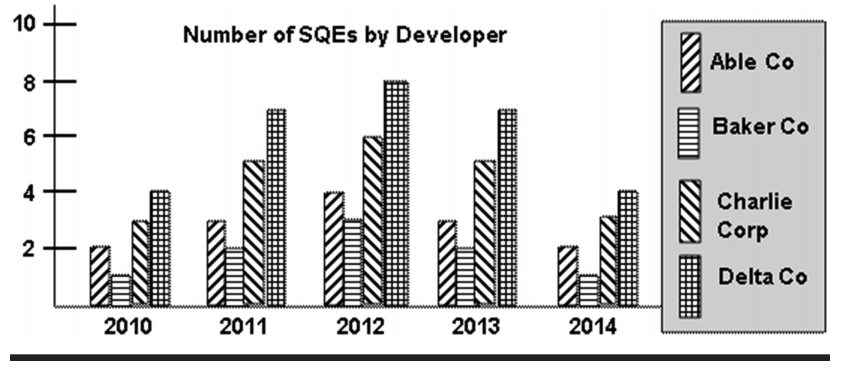
\includegraphics[width=0.95\linewidth]{1}
	\end{center}
	\caption*{\textbf{Figure 6.3 SQe staffing projection.}}
\end{figure}

SQEs work directly with their assigned Development
Teams to resolve identified problems at the lowest level
before elevating them for resolution at a higher management
level. SQEs also identify SQA tasks and responsibilities to be
implemented on the program. A detailed SQA audit schedule
should be provided in the Software Quality Program Plan
(SQPP) (see next paragraph) in terms of the SQE staffing
projections over the life of the program at each Software
Developer site as illustrated in example Figure 6.3.



\textbf{Software Quality Program Plan. }Identification of the
evaluations to be performed and the criteria to be used for
those evaluations should be defined and described in a SQPP
or similar document. This plan is normally prepared by SQA
to direct the SQE, and the SQE Team if there is more than
one SQE, in performing the evaluations. SQE tools, techniques,
 and methodologies to be employed by each software
Development Team member should also be defined in the
SQPP and can be augmented by the subsystems in their SDP
Annexes if necessary.

The SQPP is maintained and updated as needed and is
usually an addendum to the Software Development Plan. In
addition to a complete description of the evaluations to be
performed and the criteria to be used for those evaluations in
the SQPP, SQA planning should also be addressed from an
overview perspective in the SDP.


\subsubsection*{6.2.2 $\,$ Software Process Audits\\{\color{white}.} $\qquad$ and Process Reviews}
Both the subsystem level and the program-level SQA organizations perform two major types of evaluations, process
audits and product reviews:
\begin{itemize}
	\item [$\blacksquare$]
	Process audits are conducted by SQA to assure effective
	implementation of the software development process
	as defined in the SDP.
	\item [$\blacksquare$]
	Product reviews are performed by program and subsystem level SQAs as a participant in formal reviews.
	SQA product reviews verify that the software products
	conform to system requirements. Software product
	evaluations are discussed in more depth in Subsection
	6.5.6. The SQA organization should conduct ongoing
	evaluations, in accordance with the contract and the
	SDP, to ensure:
\begin{itemize}
	\item 
	Adherence of the software development processes,
	software work products, and software services to
	their applicable process descriptions, standards and
	procedures.
	\item
	That each required software product does exist, and
	that it has undergone Software Peer Reviews and
	product evaluations, testing (when applicable),
	and Corrective Actions (for identified problems).
\end{itemize}
\end{itemize}

\subsubsection*{6.2.3 $\,$ Software Quality Factors}
The subject of software quality is much broader than the
tendency to focus on software discrepancies and failure
statistics. Evaluating the quality of developmental software
products requires a “big picture” perspective. There are a
number of quality models that present ways to tie together
the different quality attributes. Table 6.4 is my succinct list
of key software quality factors plus a brief definition of each
quality factor and its related attributes.
\subsubsection*{6.2.4 $\,$ Software Quality Assurance Records}
The SQA group must maintain records for all evaluations
performed in order to provide objective evidence that the
evaluations were conducted. The records should consist of
observations or formal findings along with their resultant
Corrective Actions, disposition, metrics and closure. These
records and reports must be retained in a repository for the
duration of the contract and made available to the customer
and management as required by the contract.

Technical and management performance data should be
collected and organized into a process database. These data
should be analyzed by either SQA or the SEPG, or both, to
determine performance trends, and areas for potential process improvement. An essential element of technical performance data is the collection and analysis of measurements
(metrics) as described in Chapter 15.

\subsubsection*{6.2.5 $\,$ Software Quality Assurance\\{\color{white}.} $\qquad$ Independence}

Software Quality Engineers support software development
as an active member of the subsystem they are supporting.
However, SQEs must maintain a direct reporting line to
their SQA organization and not be in a direct reporting line
to the program they are supporting. The SDP must make it
clear that the SQE responsible for conducting the Software
Quality Assurance evaluation must not be the person who
developed, or is responsible for, the software work product.
The SQE responsible for assuring compliance with the contract must have the resources, authority and organizational
freedom to permit objective SQA evaluations and to initiate
and verify the Corrective Actions needed.

Independence in SQA is obtained by having a separate
reporting chain to Product Assurance management. If SQA
findings cannot be resolved at the lowest level possible, it
must be evaluated by the SQE to the next higher level of
management. Figure 6.4 is an example of a program’s independent reporting structure for SQA and the typical problem resolution interfaces as the resolution are elevated to a
higher management level. The objective is always to resolve
the problem at the lowest possible level.


\begin{table*}[!ht]
	\caption*{\textbf{Table 6.4 Key Software Quality Factors}}
\renewcommand{\arraystretch}{1.35}
\begin{center}
		\begin{tabular}{|l|l|}
		\hline
		{\color[HTML]{242021} \textbf{Quality Factors}} & {\color[HTML]{242021} \textbf{Definitions of the Software Quality Factors}}                                                                                                                                                                                                                                                         \\ \hline
		{\color[HTML]{242021} Correctness}              & {\color[HTML]{242021} \begin{tabular}[c]{@{}l@{}}A key attribute indicating if the software conforms to the user requirements and system\\ performance. Related attributes include: Accuracy, Completeness; Interoperability,\\  Suitability, Functionality, Verifiability; Security; Traceability and Consistency\end{tabular}}    \\ \hline
		{\color[HTML]{242021} Efficiency}               & {\color[HTML]{242021} \begin{tabular}[c]{@{}l@{}}How well the software utilizes resources in terms of its performance versus the \\ amount of planned resources to be used. Related attributes include: Accessibility\\ , Accountability, and efficiency of interfaces with peripheral devices.\end{tabular}}                       \\ \hline
		{\color[HTML]{242021} Interoperability}         & {\color[HTML]{242021} \begin{tabular}[c]{@{}l@{}}How well the software interfaces with other required operational systems. Related\\  attributes include: Modularity, Simplicity, and Data and Communications Commonality\end{tabular}}                                                                                             \\ \hline
		{\color[HTML]{242021} Maintainability}          & {\color[HTML]{242021} \begin{tabular}[c]{@{}l@{}}How easy is it to modify and upgrade the capabilities of the software. Related attributes\\  include:\\ Expandability, Flexibility, Testability, Stability, Consistency, Simplicity, Conciseness,\\  Modularity, and Self-Descriptiveness.\end{tabular}}                           \\ \hline
		{\color[HTML]{242021} Portability}              & {\color[HTML]{242021} \begin{tabular}[c]{@{}l@{}}Ability of the software to be transported from one environment to another. Related\\  attributes include: Adaptability, Installability, Replaceability, Reusability, Conformance, \\ Modularity, and System Independence.\end{tabular}}                                            \\ \hline
		{\color[HTML]{242021} Reliability}              & {\color[HTML]{242021} \begin{tabular}[c]{@{}l@{}}Capability of the software to maintain its performance level under stated conditions for\\  the required length of time. Related attributes include: Integrity, Functionality, Maturity,\\  Accuracy, Completeness, Consistency, Simplicity, and Error Tolerance.\end{tabular}}    \\ \hline
		{\color[HTML]{242021} Survivability}            & {\color[HTML]{242021} \begin{tabular}[c]{@{}l@{}}How well the software performs under all environmental conditions. Related attributes\\  include: Reliability, Portability, Interoperability and Maintainability\end{tabular}}                                                                                                     \\ \hline
		{\color[HTML]{242021} Testability}              & {\color[HTML]{242021} \begin{tabular}[c]{@{}l@{}}Ease and ability of the software to effectively test its system requirements. Related\\  attributes include: Accessibility, Communicativeness, Simplicity of the Structure, \\ Self-Descriptiveness, Instrumentation, Portability, Modularity and Stress Testability\end{tabular}} \\ \hline
		{\color[HTML]{242021} Usability}                & {\color[HTML]{242021} \begin{tabular}[c]{@{}l@{}}From a human engineering perspective, how easy the software is to use and\\  understand. Related attributes include: Learnability, Operability, Robustness, \\ Understandability, Accessibility, Training, Communicativeness, and Input/Output\\  Efficiency.\end{tabular}}        \\ \hline
	\end{tabular}
\end{center}

\end{table*}


\begin{figure*}[!ht]
	\begin{center}
		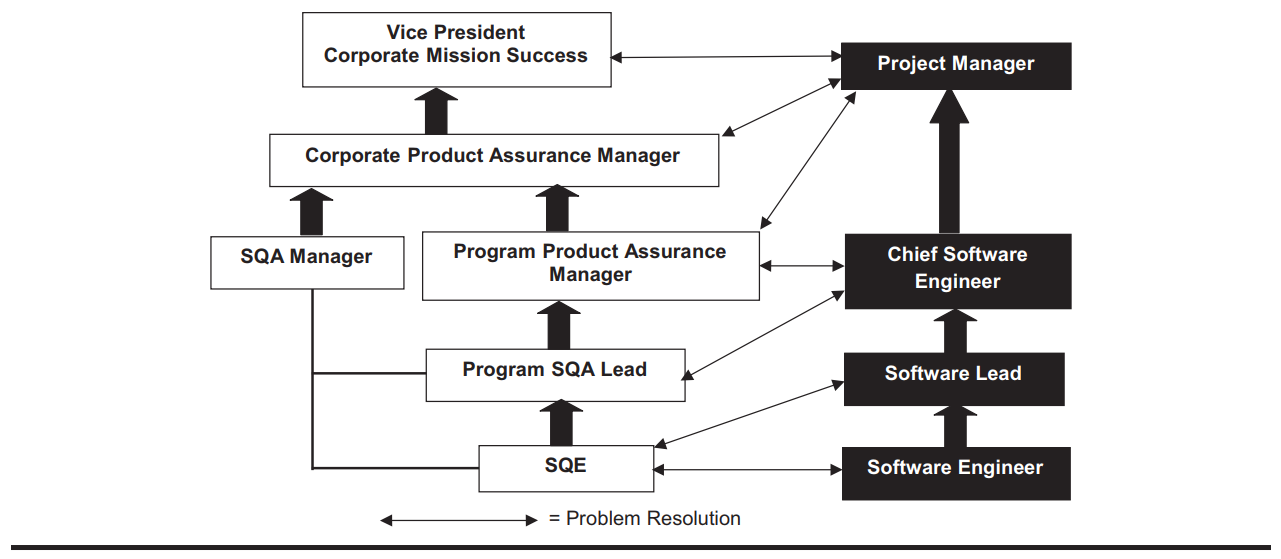
\includegraphics[width=0.9\linewidth]{2}
	\end{center}
	\caption*{\textbf{Figure 6.4 SQA independent reporting and resolution structure.}}
\end{figure*}

\subsubsection*{6.2.5 $\,$ Software Quality Assurance\\{\color{white}.} $\qquad$ Non-Compliance Issues}

All non-compliance issues, identified through audits, reviews,
normal SQA monitoring, ad-hoc findings, etc., are candidates for Corrective Action or Preventive Action as described
in Section 6.4. Correction of non-compliance issues is typically handled with an automated tool, an audit database,
and an established escalation mechanism to ensure that the
appropriate level of management can resolve the issues. In
using tools, selected by the program, non-compliance issues
should be documented, tracked to resolution, and resolved
within a given time frame. The Software Quality Assurance
organization also provides metrics data to support management decision-making as detailed in either the Quantitative
Management Plan, or the Software Measurement Plan, or
both, as discussed in Chapter 15.

\subsubsection*{6.2.5 $\,$ Software Configuration\\{\color{white}.} $\qquad$ Management and Control}

Software Configuration Management is an essential development control activity that begins during requirements definition. Formal software control starts with the establishment
of the Allocated Baseline, which identifies the Software Items
(SIs) that must be formally managed in coordination with
the Configuration Control Boards described in Subsection
6.4.3. A baseline is the initial standard or measure against
which future status, progress, and changes are compared and
measured.

\vspace{0.5cm}
\begin{minipage}[right]{.4\textwidth}
\textit{SCM is responsible for all tasks necessary to control
	baselined software products and to maintain the
	current status of the baselined products throughout
	the Development Life Cycle.}
\end{minipage}
\vspace{0.5cm}




The basic Software Configuration Management responsibilities are to:
\begin{itemize}
	\item [$\blacksquare$]

Establish formal baselines of identified products and
maintain the integrity of baselines.
\begin{itemize}
\item
 Identify software configuration items (CI), components, and related products that will be placed
under Configuration Management and when that
takes place.
\item
Create and release baselines for internal use and for
delivery to the customer.
\end{itemize}
\item [$\blacksquare$]
Track and control Change Requests for the configuration items and control the changes.
\begin{itemize}
\item
Establish and maintain a Configuration
Management and change management system for
controlling software product changes.
\item
 Establish and maintain records describing configuration items and perform configuration audits
to maintain the integrity of the configuration
baselines.
\end{itemize}
\end{itemize}
The SCM activities may be performed by both the
Development Team as well as the customer’s technical representatives. A general description of the division of SCM
responsibilities is shown in Table 6.5. On government
contracts, the customer’s technical representatives may
include Systems Engineering Technical Advisors (SETAs)
or Federally Funded Research and Development Centers
(FFRDC). On non-government contracts, the customer
technical representatives may include customer employees,
customer consultants, end-users of the system, or possibly
some stakeholders.


\begin{table}[!ht]
\caption*{\textbf{Table 6.5 Division of SCM Responsibilities}}
\begin{center}
		\begin{tabular}{|l|l|}
			\hline
			{\color[HTML]{242021} \textbf{Development team}}                                                                                            & {\color[HTML]{242021} \textbf{\begin{tabular}[c]{@{}l@{}}Customer technical\\ Representative\end{tabular}}}                                                                       \\ \hline
			{\color[HTML]{242021} \begin{tabular}[c]{@{}l@{}}Defines and\\ documents Software\\ Configuration\\ Management\\  processes\end{tabular}}   & {\color[HTML]{242021} \begin{tabular}[c]{@{}l@{}}Reviews software \\ processes for quality\\  and ensures\\ process compliance\end{tabular}}                                      \\ \hline
			{\color[HTML]{242021} \begin{tabular}[c]{@{}l@{}}Implements Software\\ Configuration\\ Management\\  tools and\\ environments\end{tabular}} & {\color[HTML]{242021} \begin{tabular}[c]{@{}l@{}}Reviews Software\\ Configuration\\  Management tools \\ and  environments for \\ quality and process \\ compliance\end{tabular}} \\ \hline
			{\color[HTML]{242021} \begin{tabular}[c]{@{}l@{}}Conducts SCM\\  boards\end{tabular}}                                                       & {\color[HTML]{242021} \begin{tabular}[c]{@{}l@{}}Participates in Software\\ Configuration \\ Management boards\end{tabular}}                                                      \\ \hline
			{\color[HTML]{242021} \begin{tabular}[c]{@{}l@{}}Ensures the\\  integrity of\\ all software\\ configuration items\end{tabular}}             & {\color[HTML]{242021} \begin{tabular}[c]{@{}l@{}}Audits delivered software\\ products for baseline \\ integrity\end{tabular}}                                                     \\ \hline
			& {\color[HTML]{242021} \begin{tabular}[c]{@{}l@{}}Incentivizes the \\ Developer to control\\  software baselines\end{tabular}}                                                     \\ \hline
		\end{tabular}
\end{center}

\end{table}

\begin{figure*}{}
	\begin{center}
		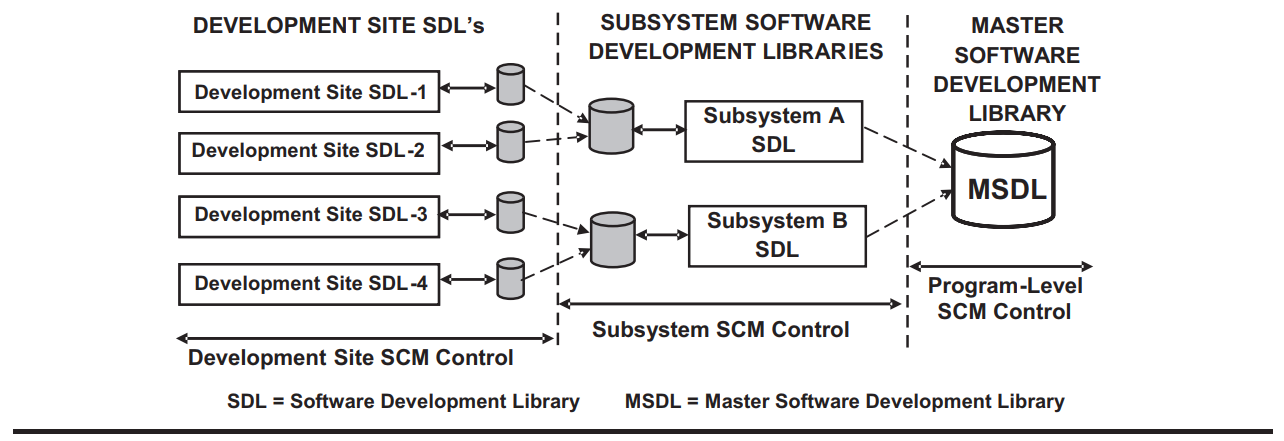
\includegraphics[width=0.9\linewidth]{3}
	\end{center}
	\caption{\textbf{Figure 6.5 Relationship of the SDLs to the MSDL.}}
\end{figure*}

Details of the SCM activity must be covered either
in the SDP, in an addendum to the SDP, or in a Software
Configuration Management Plan (SCMP). A good option is to
include an SCM overview in the SDP with the details documented in the SCMP. The SCMP is described in Subsection
6.3.4. The importance of an effective Configuration
Management process cannot be overemphasized—especially
on large projects. If program or project software is being
developed at multiple worldwide sites, the importance of
good Configuration Management is even more critical to
success.



Software Configuration Management activities are
described in the following Subsections:



\begin{itemize}
	\item [$\blacksquare$]
	 Configuration Management Control Levels: The
three-tiered SCM scheme (6.3.1)
\item [$\blacksquare$]
 Formal Baselines: Tracking versions of controlled software source code (6.3.2)
\item [$\blacksquare$]
 Software Configuration Identification: Identifying
software products under control (6.3.3)
\item [$\blacksquare$]
 Software Configuration Control: Controlling modifications to baselined products (6.3.4)
\item [$\blacksquare$]
Software Configuration Status Accounting:
Configuration status records (6.3.5)
\item [$\blacksquare$]
 Software Configuration Audits: Configuration audits
to verify changes (6.3.6)
\item [$\blacksquare$]
 Packaging, Storage, Handling and Delivery:
Preparation for system delivery (6.3.7)
\end{itemize}




\subsubsection*{6.2.5 $\,$ Software Configuration\\{\color{white}.} $\qquad$ Management Control Levels}

Typically, SCM has a three-tiered Configuration Management
control scheme as shown in Figure 6.5. It consists of a program-level, subsystem level, and development site control of
software libraries.





SCM tasks should be performed at each software development site utilizing the site’s Software Development Library
(SDL) for configuration control of the developed products.
On large programs, the SDLs are typically subdivided into
two levels—at the Developer level and at the element or subsystem level, as shown in Figure 6.5. The software products
move up the levels to until they reach the program’s Master
Software Development Library (MSDL). The development
and subsystem sites may be co-located.

SCM establishes and maintains the integrity of specified
software work products, controls and promotes stable baselines, maintains status accounting of the baselines throughout the life of a project, and controls the build process
through product delivery. Responsibility for SCM should
reside with the Software Group Lead. The principal SCM
performers within subsystem and development sites are the
SCM Lead and the SCM Librarian.


\textbf{Library Levels.} The specific organization of the SDL and
MSDL must be tailored to each program; however, Table 6.6 is
an example of the library levels, names, and who controls them.
Specific guidance regarding structure and control of the
software libraries should be provided in the SDP and/or the
SCMP. A discussion of Software Development Libraries,
source code version control, and electronic SDL file partitioning is addressed in Section 9.3.



\subsubsection*{6.3.2 $\,$ Formal Baselines}
Baselines are initial standards or product versions against
which future status, progress, and changes are compared and
measured. The budget and schedule can serve as baselines.
Software baselines change and become specific versions of
controlled requirements, source code, build files, user documentation or data for an increment, build, or release. A brief
comparison of the differences between the various software
baselines is shown in Table 6.7. A requirements baseline
involves an approved Software Requirements Specification
(SRS) under SCM control.



\textbf{Software Version Control.} Version control, also called
revision or source control, involves the management of
changes to source code, documentation and other collections
of information. It is an important component of Software
Configuration Management because it is common for multiple versions of the same software, or documentation, to be
deployed in different sites and for Software Developers to be



\end{document}